\documentclass[crop,tikz]{standalone}

\usepackage{amsmath}
\newcommand{\F}{\vec{F}}
\newcommand{\place}{\vec{r}}
\tikzset{>=latex}
\usetikzlibrary{calc,patterns,decorations.pathmorphing}
\colorlet{green}{black!40!green}

\begin{document}
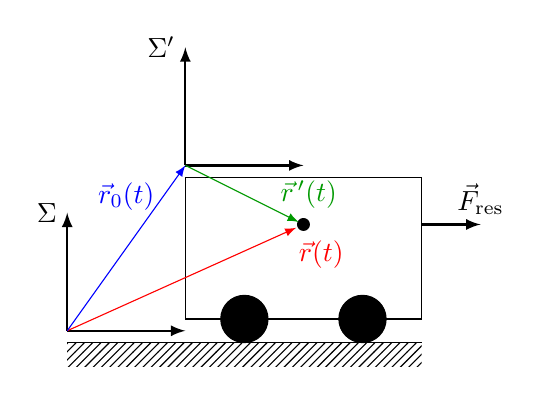
\begin{tikzpicture}[scale=1.5]
  \pattern[pattern=north east lines,pattern color=black] (0,0)--++(3,0)--++(0,-0.2)--++(-3,0)--cycle;
  \draw (0,0) -- (3,0);
  \draw[->,thick] (3,1) -- +(0.5,0) node[above]{$\F_\text{res}$};
  % Sigma
  \coordinate (s) at (0,0.1);
  \draw[->,thick] (s) -- +(1,0);
  \draw[->,thick] (s) -- +(0,1) node[left] {$\Sigma$};
  % car
  \draw (1,0.2) rectangle (3,1.4);
  \draw[fill] (1.5,0.2) circle (0.2);
  \draw[fill] (2.5,0.2) circle (0.2);
  % Sigma'
  \coordinate (sp) at (1,1.5);
  \draw[->,thick] (sp) -- +(1,0);
  \draw[->,thick] (sp) -- +(0,1) node[left] {$\Sigma'$};
  % r
  \coordinate (m) at (2,1);
  \draw[fill,black] (m) circle (0.05);
  \draw[->,red,shorten >= 1]   (s)  -- node[above,xshift=5em] {$\place(t)$} ($(s)!0.98!(m)$);
  \draw[->,green,shorten >= 1] (sp) -- node[right,xshift=1em] {$\place^{\,\prime}(t)$} ($(sp)!0.98!(m)$);
  \draw[->,blue]  (s)  -- node[above,yshift=1em] {$\place_0(t)$} (sp);
\end{tikzpicture}
\end{document}
